\documentclass{article}
\usepackage[utf8]{inputenc}
\usepackage[T5]{fontenc}
\usepackage{graphicx}
\usepackage[margin=2cm]{geometry}
\title{Report 7: Grayscale Stretch}
\author{Nguyễn Thanh Hùng -- 2540056}
\date{}

\begin{document}
\maketitle

\section{Implementation}
I used two CUDA reductions to find the minimum and maximum grayscale values. A 2D kernel then computes $(p-\min)255/(\max-\min)$. Constant images are kept unchanged to avoid division by zero. I checked the extrema and output against NumPy.

I ran the notebook on Google Colab with a Tesla T4 and a $256\times256$ sample image.
GPU timings use \texttt{time.time()} after warm-up and synchronization, averaged over three runs; allocation and image transfers are excluded. Where measured, CPU time is one run; speedup is relative to that Python CPU implementation.

\section{Results}
Input minimum/maximum: 2/250; output: 0/255. Maximum pixel error: 0.

Reduction time: 0.9581 ms, including returning the two scalars to the host.
\begin{center}
\begin{tabular}{lr}
\hline
Block & Stretch kernel (ms) \\
\hline
(8, 8) & 0.0718 \\
(16, 16) & 0.0548 \\
(32, 16) & 0.0558 \\
(32, 32) & 0.0481 \\
\hline
\end{tabular}
\end{center}\begin{center}
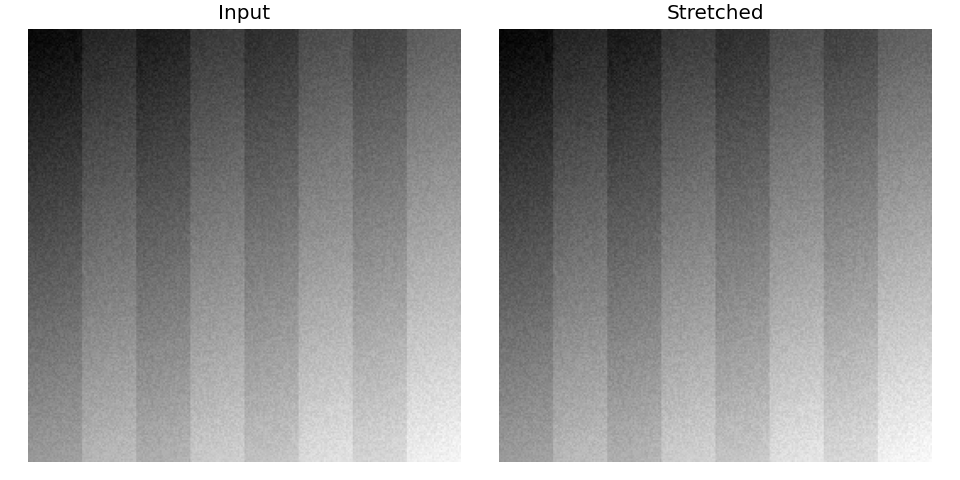
\includegraphics[width=.85\linewidth,height=.19\textheight,keepaspectratio]{figures/images.png}
\end{center}

\section{Discussion}
The output uses the full grayscale range. The $32\times32$ block gave the lowest map time (0.0481 ms). Finding the extrema took much longer than the pixel mapping on this small image.

\end{document}
